\newcommand{\arcanaDescription}{
\section{Arcana}
\epigraph{\textit{
    "So what if the land becomes barren? It’s not like we're going to stick around."
} }{
    Datuu Dawnchaser, Elf Defiler
}

    Athasian wizards drain energy from the surrounding
    soil. The method used labels the wizard as a defiler or a
    preserver. Preservers have the self-control to gather
    energy without destroying plants. Those who do not, or
    who feel no remorse about the damage caused, become
    Defilers. Defilers leave behind sterile soil and infertile ash
    when they cast spells. Because of this, most wastelanders
    blame wizards for the desert landscape that dominates
    the Tablelands today, and their hatred extends to defilers
    and preservers alike. In the seven cities, arcana magic is\\
    outlawed and feared.\\
    Writing is also illegal in the Tablelands, thus wizards
    have to go to great lengths to conceal their spellbooks,
    and they have refined this art to the point where even
    fellow wizards can be hard pressed to identify a spell
    book. When found, they are precious resources, hoarded
    and studied by wizards thirsty for knowledge or power.\\
    \\
    See \nref{tlttree:arcana} for more information.
}

\newcommand{\arcanaTree}{
    \newpage
    \subsection{Arcana Talent Tree}
    \label{tlttree:arcana}

    \textbf{Class Skills:} Arcana, Deception, Alchemy, Vigilance
    \newline

    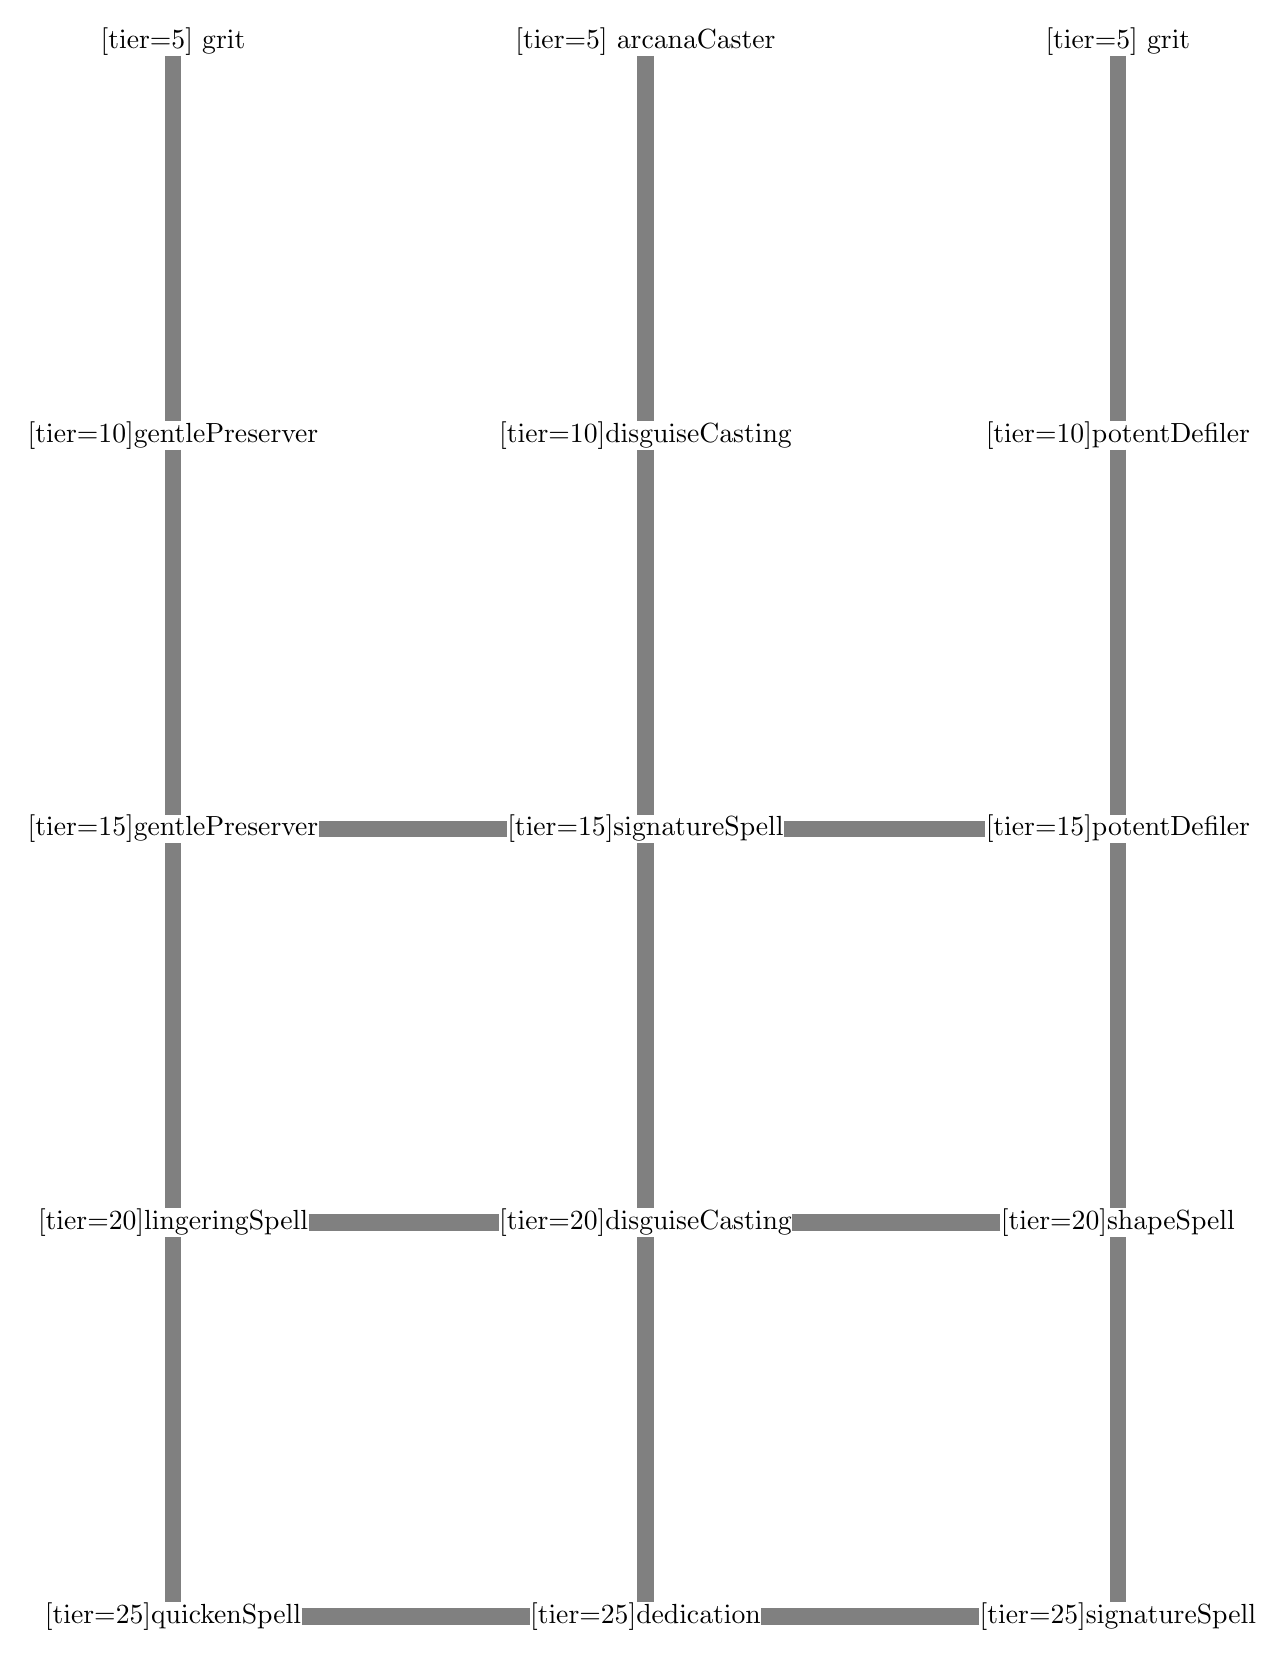
\begin{tikzpicture}
        \draw ( 0,  0) node(aa)[inner sep=0]{\TalentBox[tier=5] {grit}}
              ( 6,  0) node(ab)[inner sep=0]{\TalentBox[tier=5] {arcanaCaster}}
              (12,  0) node(ac)[inner sep=0]{\TalentBox[tier=5] {grit}}
              ( 0, -5) node(ba)[inner sep=0]{\TalentBox[tier=10]{gentlePreserver}}
              ( 6, -5) node(bb)[inner sep=0]{\TalentBox[tier=10]{disguiseCasting}}
              (12, -5) node(bc)[inner sep=0]{\TalentBox[tier=10]{potentDefiler}}
              ( 0,-10) node(ca)[inner sep=0]{\TalentBox[tier=15]{gentlePreserver}}
              ( 6,-10) node(cb)[inner sep=0]{\TalentBox[tier=15]{signatureSpell}}
              (12,-10) node(cc)[inner sep=0]{\TalentBox[tier=15]{potentDefiler}}
              ( 0,-15) node(da)[inner sep=0]{\TalentBox[tier=20]{lingeringSpell}}
              ( 6,-15) node(db)[inner sep=0]{\TalentBox[tier=20]{disguiseCasting}}
              (12,-15) node(dc)[inner sep=0]{\TalentBox[tier=20]{shapeSpell}}
              ( 0,-20) node(ea)[inner sep=0]{\TalentBox[tier=25]{quickenSpell}}
              ( 6,-20) node(eb)[inner sep=0]{\TalentBox[tier=25]{dedication}}
              (12,-20) node(ec)[inner sep=0]{\TalentBox[tier=25]{signatureSpell}}
        ;

        \tikzstyle{bar}=[gray,-,>=stealth, line width=6pt]

        \draw [bar] (aa) edge (ba);
        \draw [bar] (ab) edge (bb);
        \draw [bar] (ac) edge (bc);

        \draw [bar] (ba) edge (ca);
        \draw [bar] (bb) edge (cb);
        \draw [bar] (bc) edge (cc);

        \draw [bar] (ca) edge (da);
        \draw [bar] (cb) edge (db);
        \draw [bar] (cc) edge (dc);

        \draw [bar] (da) edge (ea);
        \draw [bar] (db) edge (eb);
        \draw [bar] (dc) edge (ec);

        \draw [bar] (ca) edge (cb);
        \draw [bar] (cc) edge (cb);

        \draw [bar] (da) edge (db);
        \draw [bar] (dc) edge (db);

        \draw [bar] (ea) edge (eb);
        \draw [bar] (ec) edge (eb);
    \end{tikzpicture}
}
